\documentclass{standalone}
\usepackage{tikz}
\usetikzlibrary{patterns, positioning}

\begin{document}
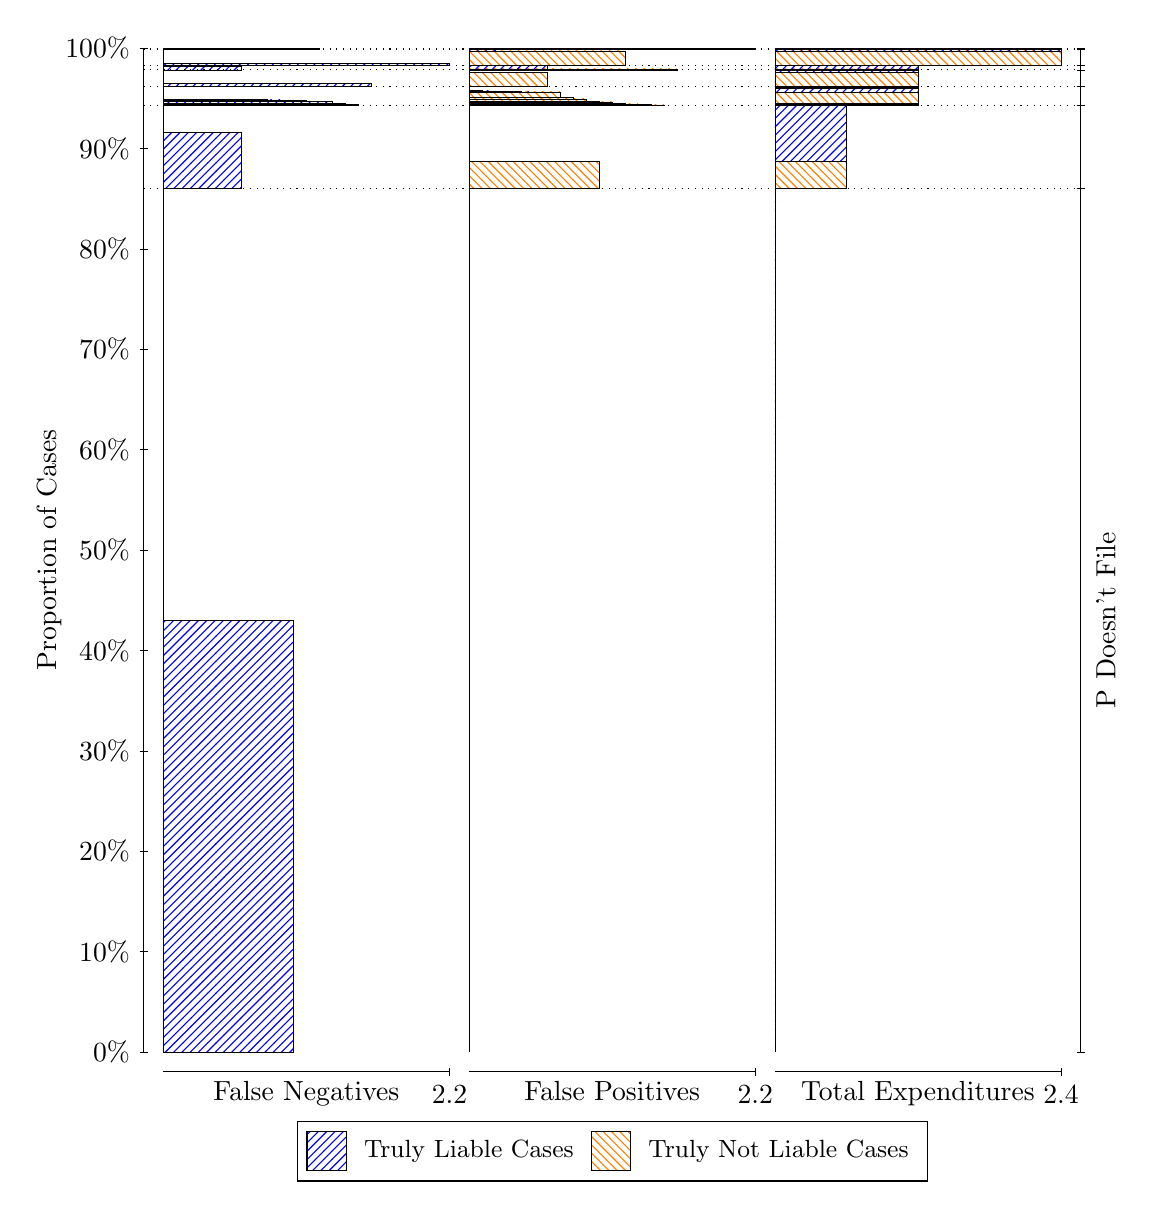
\begin{tikzpicture}
\draw[black, very thin] (1.5,1.75) -- (1.5,14.5);
\node[rotate=90, anchor=center] at (0.3, 8.125) {Proportion of Cases};
\draw[black, very thin] (1.45,1.75) -- (1.55,1.75);
\node[anchor=east] at (1.45, 1.75) {0\%};
\draw[black, very thin] (1.45,3.025) -- (1.55,3.025);
\node[anchor=east] at (1.45, 3.025) {10\%};
\draw[black, very thin] (1.45,4.3) -- (1.55,4.3);
\node[anchor=east] at (1.45, 4.3) {20\%};
\draw[black, very thin] (1.45,5.575) -- (1.55,5.575);
\node[anchor=east] at (1.45, 5.575) {30\%};
\draw[black, very thin] (1.45,6.85) -- (1.55,6.85);
\node[anchor=east] at (1.45, 6.85) {40\%};
\draw[black, very thin] (1.45,8.125) -- (1.55,8.125);
\node[anchor=east] at (1.45, 8.125) {50\%};
\draw[black, very thin] (1.45,9.4) -- (1.55,9.4);
\node[anchor=east] at (1.45, 9.4) {60\%};
\draw[black, very thin] (1.45,10.675) -- (1.55,10.675);
\node[anchor=east] at (1.45, 10.675) {70\%};
\draw[black, very thin] (1.45,11.95) -- (1.55,11.95);
\node[anchor=east] at (1.45, 11.95) {80\%};
\draw[black, very thin] (1.45,13.225) -- (1.55,13.225);
\node[anchor=east] at (1.45, 13.225) {90\%};
\draw[black, very thin] (1.45,14.5) -- (1.55,14.5);
\node[anchor=east] at (1.45, 14.5) {100\%};

\draw[black, very thin] (13.4,1.75) -- (13.4,14.5);
\draw[black, very thin] (13.35,1.75) -- (13.45,1.75);
\node[anchor=west] at (13.35, 1.75) {};
\draw[black, very thin] (13.35,12.719) -- (13.45,12.719);
\node[anchor=west] at (13.35, 12.719) {};
\draw[black, very thin] (13.35,13.775) -- (13.45,13.775);
\node[anchor=west] at (13.35, 13.775) {};
\draw[black, very thin] (13.35,14.013) -- (13.45,14.013);
\node[anchor=west] at (13.35, 14.013) {};
\draw[black, very thin] (13.35,14.222) -- (13.45,14.222);
\node[anchor=west] at (13.35, 14.222) {};
\draw[black, very thin] (13.35,14.278) -- (13.45,14.278);
\node[anchor=west] at (13.35, 14.278) {};
\draw[black, very thin] (13.35,14.487) -- (13.45,14.487);
\node[anchor=west] at (13.35, 14.487) {};
\draw[black, very thin] (13.35,14.5) -- (13.45,14.5);
\node[anchor=west] at (13.35, 14.5) {};

\draw[black, very thin, pattern color=blue, pattern=north east lines] (1.75,1.75) rectangle (3.4015,7.2346);
\draw[black, very thin, pattern color=orange, pattern=north west lines] (1.75,7.2346) rectangle (1.75,12.719);
\draw[black, very thin, pattern color=blue, pattern=north east lines] (1.75,12.719) rectangle (2.7409,13.431);
\draw[black, very thin, pattern color=orange, pattern=north west lines] (1.75,13.431) rectangle (1.75,13.775);
\draw[black, very thin, pattern color=blue, pattern=north east lines] (1.75,13.775) rectangle (4.2273,13.787);
\draw[black, very thin, pattern color=blue, pattern=north east lines] (1.75,13.787) rectangle (4.0621,13.801);
\draw[black, very thin, pattern color=blue, pattern=north east lines] (1.75,13.801) rectangle (3.897,13.819);
\draw[black, very thin, pattern color=blue, pattern=north east lines] (1.75,13.819) rectangle (3.7318,13.824);
\draw[black, very thin, pattern color=blue, pattern=north east lines] (1.75,13.824) rectangle (3.5667,13.831);
\draw[black, very thin, pattern color=blue, pattern=north east lines] (1.75,13.831) rectangle (3.4015,13.836);
\draw[black, very thin, pattern color=blue, pattern=north east lines] (1.75,13.836) rectangle (3.2364,13.841);
\draw[black, very thin, pattern color=blue, pattern=north east lines] (1.75,13.841) rectangle (3.0712,13.843);
\draw[black, very thin, pattern color=blue, pattern=north east lines] (1.75,13.843) rectangle (2.9061,13.845);
\draw[black, very thin, pattern color=orange, pattern=north west lines] (1.75,13.845) rectangle (1.75,14.013);
\draw[black, very thin, pattern color=blue, pattern=north east lines] (1.75,14.013) rectangle (4.3924,14.049);
\draw[black, very thin, pattern color=orange, pattern=north west lines] (1.75,14.049) rectangle (1.75,14.222);
\draw[black, very thin, pattern color=blue, pattern=north east lines] (1.75,14.222) rectangle (2.7409,14.265);
\draw[black, very thin, pattern color=orange, pattern=north west lines] (1.75,14.265) rectangle (1.75,14.278);
\draw[black, very thin, pattern color=blue, pattern=north east lines] (1.75,14.278) rectangle (5.3833,14.3);
\draw[black, very thin, pattern color=orange, pattern=north west lines] (1.75,14.3) rectangle (1.75,14.487);
\draw[black, very thin, pattern color=blue, pattern=north east lines] (1.75,14.487) rectangle (3.7318,14.495);
\draw[black, very thin, pattern color=orange, pattern=north west lines] (1.75,14.495) rectangle (1.75,14.5);
\draw[black, very thin, pattern color=orange, pattern=north west lines] (5.6333,1.75) rectangle (5.6333,7.2346);
\draw[black, very thin, pattern color=blue, pattern=north east lines] (5.6333,7.2346) rectangle (5.6333,12.719);
\draw[black, very thin, pattern color=orange, pattern=north west lines] (5.6333,12.719) rectangle (7.2848,13.063);
\draw[black, very thin, pattern color=blue, pattern=north east lines] (5.6333,13.063) rectangle (5.6333,13.775);
\draw[black, very thin, pattern color=orange, pattern=north west lines] (5.6333,13.775) rectangle (8.1106,13.779);
\draw[black, very thin, pattern color=orange, pattern=north west lines] (5.6333,13.779) rectangle (7.9455,13.783);
\draw[black, very thin, pattern color=orange, pattern=north west lines] (5.6333,13.783) rectangle (7.7803,13.791);
\draw[black, very thin, pattern color=orange, pattern=north west lines] (5.6333,13.791) rectangle (7.6152,13.8);
\draw[black, very thin, pattern color=orange, pattern=north west lines] (5.6333,13.8) rectangle (7.45,13.815);
\draw[black, very thin, pattern color=orange, pattern=north west lines] (5.6333,13.815) rectangle (7.2848,13.825);
\draw[black, very thin, pattern color=orange, pattern=north west lines] (5.6333,13.825) rectangle (7.1197,13.854);
\draw[black, very thin, pattern color=orange, pattern=north west lines] (5.6333,13.854) rectangle (6.9545,13.874);
\draw[black, very thin, pattern color=orange, pattern=north west lines] (5.6333,13.874) rectangle (6.7894,13.942);
\draw[black, very thin, pattern color=blue, pattern=north east lines] (5.6333,13.942) rectangle (6.4591,13.944);
\draw[black, very thin, pattern color=blue, pattern=north east lines] (5.6333,13.944) rectangle (6.2939,13.947);
\draw[black, very thin, pattern color=blue, pattern=north east lines] (5.6333,13.947) rectangle (6.1288,13.952);
\draw[black, very thin, pattern color=blue, pattern=north east lines] (5.6333,13.952) rectangle (5.9636,13.957);
\draw[black, very thin, pattern color=blue, pattern=north east lines] (5.6333,13.957) rectangle (5.7985,13.964);
\draw[black, very thin, pattern color=blue, pattern=north east lines] (5.6333,13.964) rectangle (5.6333,14.013);
\draw[black, very thin, pattern color=orange, pattern=north west lines] (5.6333,14.013) rectangle (6.6242,14.186);
\draw[black, very thin, pattern color=blue, pattern=north east lines] (5.6333,14.186) rectangle (5.6333,14.222);
\draw[black, very thin, pattern color=orange, pattern=north west lines] (5.6333,14.222) rectangle (8.2758,14.236);
\draw[black, very thin, pattern color=blue, pattern=north east lines] (5.6333,14.236) rectangle (6.6242,14.278);
\draw[black, very thin, pattern color=orange, pattern=north west lines] (5.6333,14.278) rectangle (7.6152,14.465);
\draw[black, very thin, pattern color=blue, pattern=north east lines] (5.6333,14.465) rectangle (5.9636,14.487);
\draw[black, very thin, pattern color=orange, pattern=north west lines] (5.6333,14.487) rectangle (9.2667,14.492);
\draw[black, very thin, pattern color=blue, pattern=north east lines] (5.6333,14.492) rectangle (7.6152,14.5);
\draw[black, very thin, pattern color=orange, pattern=north west lines] (9.5167,1.75) rectangle (9.5167,7.2346);
\draw[black, very thin, pattern color=blue, pattern=north east lines] (9.5167,7.2346) rectangle (9.5167,12.719);
\draw[black, very thin, pattern color=orange, pattern=north west lines] (9.5167,12.719) rectangle (10.425,13.063);
\draw[black, very thin, pattern color=blue, pattern=north east lines] (9.5167,13.063) rectangle (10.425,13.775);
\draw[black, very thin, pattern color=orange, pattern=north west lines] (9.5167,13.775) rectangle (11.333,13.79);
\draw[black, very thin, pattern color=blue, pattern=north east lines] (9.5167,13.79) rectangle (11.333,13.797);
\draw[black, very thin, pattern color=orange, pattern=north west lines] (9.5167,13.797) rectangle (11.333,13.937);
\draw[black, very thin, pattern color=blue, pattern=north east lines] (9.5167,13.937) rectangle (11.333,13.993);
\draw[black, very thin, pattern color=orange, pattern=north west lines] (9.5167,13.993) rectangle (11.333,14.005);
\draw[black, very thin, pattern color=blue, pattern=north east lines] (9.5167,14.005) rectangle (11.333,14.013);
\draw[black, very thin, pattern color=orange, pattern=north west lines] (9.5167,14.013) rectangle (11.333,14.186);
\draw[black, very thin, pattern color=blue, pattern=north east lines] (9.5167,14.186) rectangle (11.333,14.222);
\draw[black, very thin, pattern color=orange, pattern=north west lines] (9.5167,14.222) rectangle (11.333,14.236);
\draw[black, very thin, pattern color=blue, pattern=north east lines] (9.5167,14.236) rectangle (11.333,14.278);
\draw[black, very thin, pattern color=orange, pattern=north west lines] (9.5167,14.278) rectangle (13.15,14.465);
\draw[black, very thin, pattern color=blue, pattern=north east lines] (9.5167,14.465) rectangle (13.15,14.487);
\draw[black, very thin, pattern color=orange, pattern=north west lines] (9.5167,14.487) rectangle (13.15,14.492);
\draw[black, very thin, pattern color=blue, pattern=north east lines] (9.5167,14.492) rectangle (13.15,14.5);
\draw[black, dotted] (1.5,12.719) -- (13.4,12.719);
\draw[black, dotted] (1.5,13.775) -- (13.4,13.775);
\draw[black, dotted] (1.5,14.013) -- (13.4,14.013);
\draw[black, dotted] (1.5,14.222) -- (13.4,14.222);
\draw[black, dotted] (1.5,14.278) -- (13.4,14.278);
\draw[black, dotted] (1.5,14.487) -- (13.4,14.487);
\draw[black, very thin] (1.75,1.5) -- (5.3833,1.5);
\node[anchor=north] at (3.5667, 1.5) {False Negatives};
\draw[black, very thin] (5.3833,1.45) -- (5.3833,1.55);
\node[anchor=north] at (5.3833, 1.45) {2.2};

\draw[black, very thin] (5.6333,1.5) -- (9.2667,1.5);
\node[anchor=north] at (7.45, 1.5) {False Positives};
\draw[black, very thin] (9.2667,1.45) -- (9.2667,1.55);
\node[anchor=north] at (9.2667, 1.45) {2.2};

\draw[black, very thin] (9.5167,1.5) -- (13.15,1.5);
\node[anchor=north] at (11.333, 1.5) {Total Expenditures};
\draw[black, very thin] (13.15,1.45) -- (13.15,1.55);
\node[anchor=north] at (13.15, 1.45) {2.4};

\node[black, centered, rotate=90] at (13.72, 7.2346) {P Doesn't File};







\draw (7.449999999999999,1.5) node[draw=none] (baseCoordinate) {};
\begin{scope}[align=center]
        \matrix[scale=0.5, draw=black, below=0.5cm of baseCoordinate, nodes={draw}, column sep=0.1cm]{
            \node[rectangle, draw, minimum width=0.5cm, minimum height=0.5cm, pattern=north east lines, pattern color=blue] {}; &
            \node[draw=none, font=\small] (B) {Truly Liable Cases}; &
            \node[rectangle, draw, minimum width=0.5cm, minimum height=0.5cm, pattern=north west lines, pattern color=orange] {}; &
            \node[draw=none, font=\small] (B) {Truly Not Liable Cases}; \\
            };
\end{scope}

\end{tikzpicture}
\end{document}